% Created by tikzDevice version 0.12.3 on 2020-09-20 16:25:20
% !TEX encoding = UTF-8 Unicode
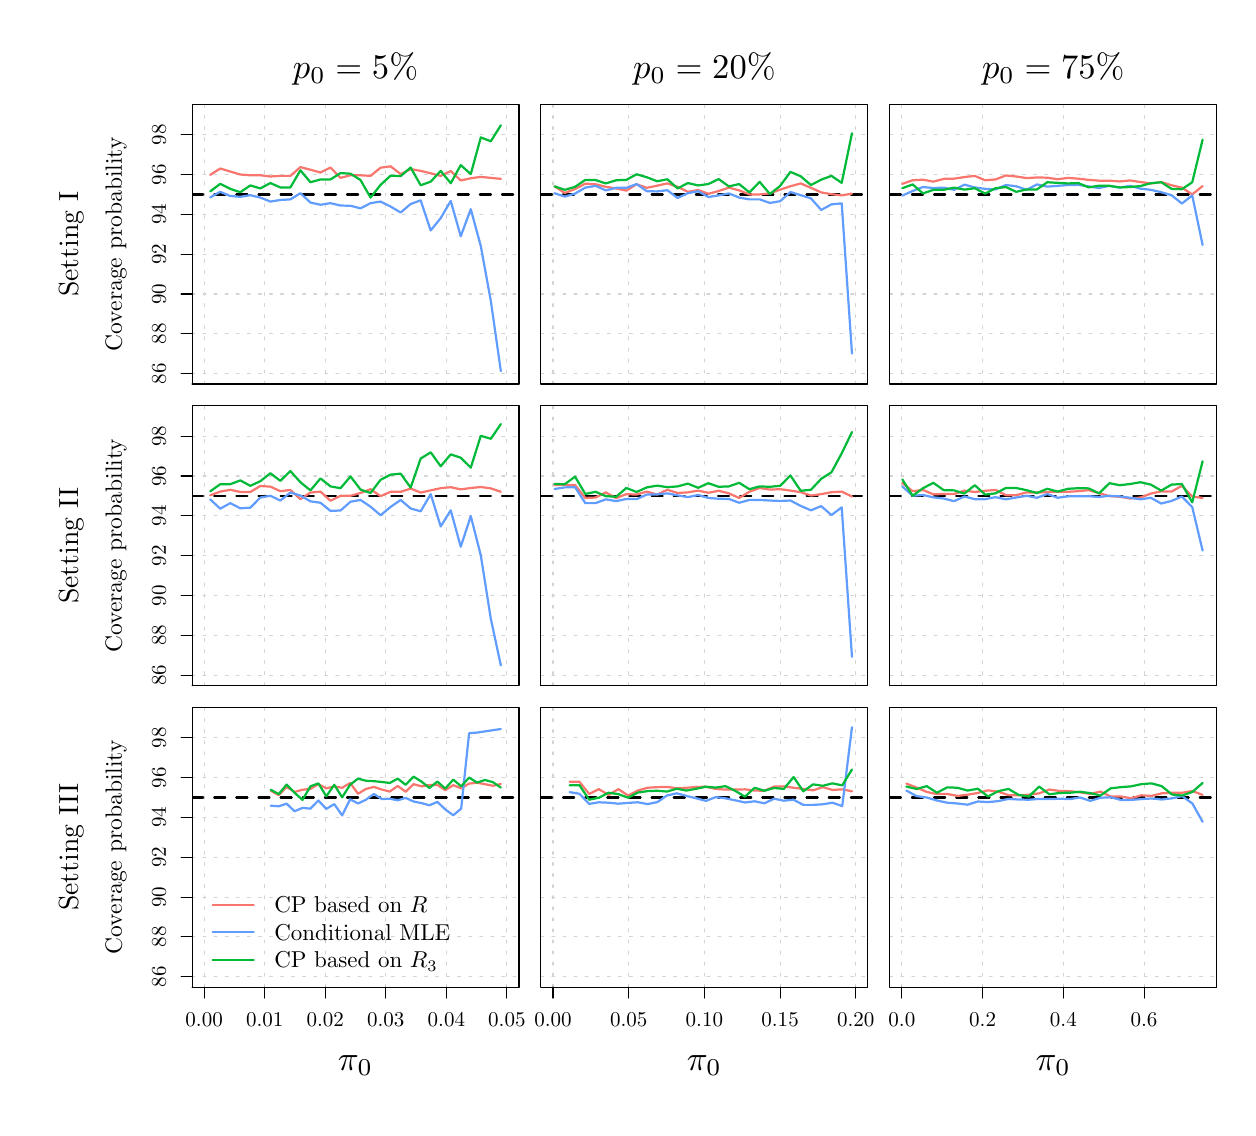
\begin{tikzpicture}[x=1pt,y=1pt]
\definecolor{fillColor}{RGB}{255,255,255}
\path[use as bounding box,fill=fillColor,fill opacity=0.00] (0,0) rectangle (433.62,390.26);
\begin{scope}
\path[clip] ( 55.44,257.53) rectangle (181.50,366.50);
\definecolor{drawColor}{RGB}{0,0,0}

\node[text=drawColor,anchor=base,inner sep=0pt, outer sep=0pt, scale=  0.66] at (118.47,231.40) {Simulation ID};

\node[text=drawColor,rotate= 90.00,anchor=base,inner sep=0pt, outer sep=0pt, scale=  0.66] at ( 34.06,312.01) {Ratio of RMSE};
\end{scope}
\begin{scope}
\path[clip] (  0.00,  0.00) rectangle (433.62,390.26);
\definecolor{drawColor}{RGB}{0,0,0}

\path[draw=drawColor,line width= 0.4pt,line join=round,line cap=round] ( 59.40,265.23) -- ( 59.40,351.60);

\path[draw=drawColor,line width= 0.4pt,line join=round,line cap=round] ( 59.40,265.23) -- ( 55.44,265.23);

\path[draw=drawColor,line width= 0.4pt,line join=round,line cap=round] ( 59.40,279.63) -- ( 55.44,279.63);

\path[draw=drawColor,line width= 0.4pt,line join=round,line cap=round] ( 59.40,294.02) -- ( 55.44,294.02);

\path[draw=drawColor,line width= 0.4pt,line join=round,line cap=round] ( 59.40,308.42) -- ( 55.44,308.42);

\path[draw=drawColor,line width= 0.4pt,line join=round,line cap=round] ( 59.40,322.81) -- ( 55.44,322.81);

\path[draw=drawColor,line width= 0.4pt,line join=round,line cap=round] ( 59.40,337.20) -- ( 55.44,337.20);

\path[draw=drawColor,line width= 0.4pt,line join=round,line cap=round] ( 59.40,351.60) -- ( 55.44,351.60);

\node[text=drawColor,rotate= 90.00,anchor=base,inner sep=0pt, outer sep=0pt, scale=  0.76] at ( 49.90,265.23) {86};

\node[text=drawColor,rotate= 90.00,anchor=base,inner sep=0pt, outer sep=0pt, scale=  0.76] at ( 49.90,279.63) {88};

\node[text=drawColor,rotate= 90.00,anchor=base,inner sep=0pt, outer sep=0pt, scale=  0.76] at ( 49.90,294.02) {90};

\node[text=drawColor,rotate= 90.00,anchor=base,inner sep=0pt, outer sep=0pt, scale=  0.76] at ( 49.90,308.42) {92};

\node[text=drawColor,rotate= 90.00,anchor=base,inner sep=0pt, outer sep=0pt, scale=  0.76] at ( 49.90,322.81) {94};

\node[text=drawColor,rotate= 90.00,anchor=base,inner sep=0pt, outer sep=0pt, scale=  0.76] at ( 49.90,337.20) {96};

\node[text=drawColor,rotate= 90.00,anchor=base,inner sep=0pt, outer sep=0pt, scale=  0.76] at ( 49.90,351.60) {98};
\end{scope}
\begin{scope}
\path[clip] ( 59.40,261.49) rectangle (177.54,362.54);
\definecolor{drawColor}{RGB}{211,211,211}

\path[draw=drawColor,line width= 0.4pt,dash pattern=on 1pt off 3pt ,line join=round,line cap=round] ( 63.78,261.49) -- ( 63.78,362.54);

\path[draw=drawColor,line width= 0.4pt,dash pattern=on 1pt off 3pt ,line join=round,line cap=round] ( 85.65,261.49) -- ( 85.65,362.54);

\path[draw=drawColor,line width= 0.4pt,dash pattern=on 1pt off 3pt ,line join=round,line cap=round] (107.53,261.49) -- (107.53,362.54);

\path[draw=drawColor,line width= 0.4pt,dash pattern=on 1pt off 3pt ,line join=round,line cap=round] (129.41,261.49) -- (129.41,362.54);

\path[draw=drawColor,line width= 0.4pt,dash pattern=on 1pt off 3pt ,line join=round,line cap=round] (151.29,261.49) -- (151.29,362.54);

\path[draw=drawColor,line width= 0.4pt,dash pattern=on 1pt off 3pt ,line join=round,line cap=round] (173.16,261.49) -- (173.16,362.54);

\path[draw=drawColor,line width= 0.4pt,dash pattern=on 1pt off 3pt ,line join=round,line cap=round] ( 59.40,265.23) -- (177.54,265.23);

\path[draw=drawColor,line width= 0.4pt,dash pattern=on 1pt off 3pt ,line join=round,line cap=round] ( 59.40,279.63) -- (177.54,279.63);

\path[draw=drawColor,line width= 0.4pt,dash pattern=on 1pt off 3pt ,line join=round,line cap=round] ( 59.40,294.02) -- (177.54,294.02);

\path[draw=drawColor,line width= 0.4pt,dash pattern=on 1pt off 3pt ,line join=round,line cap=round] ( 59.40,308.42) -- (177.54,308.42);

\path[draw=drawColor,line width= 0.4pt,dash pattern=on 1pt off 3pt ,line join=round,line cap=round] ( 59.40,322.81) -- (177.54,322.81);

\path[draw=drawColor,line width= 0.4pt,dash pattern=on 1pt off 3pt ,line join=round,line cap=round] ( 59.40,337.20) -- (177.54,337.20);

\path[draw=drawColor,line width= 0.4pt,dash pattern=on 1pt off 3pt ,line join=round,line cap=round] ( 59.40,351.60) -- (177.54,351.60);
\end{scope}
\begin{scope}
\path[clip] (  0.00,  0.00) rectangle (433.62,390.26);
\definecolor{drawColor}{RGB}{0,0,0}

\path[draw=drawColor,line width= 0.4pt,line join=round,line cap=round] ( 59.40,261.49) --
	(177.54,261.49) --
	(177.54,362.54) --
	( 59.40,362.54) --
	( 59.40,261.49);
\end{scope}
\begin{scope}
\path[clip] ( 59.40,261.49) rectangle (177.54,362.54);
\definecolor{drawColor}{RGB}{0,0,0}

\path[draw=drawColor,line width= 0.8pt,dash pattern=on 4pt off 4pt ,line join=round,line cap=round] ( 59.40,330.01) -- (177.54,330.01);
\definecolor{drawColor}{RGB}{248,118,109}

\path[draw=drawColor,line width= 0.8pt,line join=round,line cap=round] ( 65.96,337.06) --
	( 69.58,339.36) --
	( 73.21,338.28) --
	( 76.83,337.20) --
	( 80.45,336.92) --
	( 84.07,336.92) --
	( 87.69,336.48) --
	( 91.31,336.70) --
	( 94.93,336.70) --
	( 98.55,339.87) --
	(102.17,338.93) --
	(105.80,337.92) --
	(109.42,339.72) --
	(113.04,335.98) --
	(116.66,336.92) --
	(120.28,336.92) --
	(123.90,336.70) --
	(127.52,339.65) --
	(131.14,340.16) --
	(134.77,337.35) --
	(138.39,339.15) --
	(142.01,338.50) --
	(145.63,337.64) --
	(149.25,336.70) --
	(152.87,338.43) --
	(156.49,335.05) --
	(160.11,335.84) --
	(163.73,336.34) --
	(167.36,335.98) --
	(170.98,335.62);
\definecolor{drawColor}{RGB}{97,156,255}

\path[draw=drawColor,line width= 0.8pt,line join=round,line cap=round] ( 65.96,328.93) --
	( 69.58,330.94) --
	( 73.21,329.43) --
	( 76.83,329.14) --
	( 80.45,329.72) --
	( 84.07,328.86) --
	( 87.69,327.42) --
	( 91.31,327.99) --
	( 94.93,328.21) --
	( 98.55,330.44) --
	(102.17,327.06) --
	(105.80,326.27) --
	(109.42,326.84) --
	(113.04,325.98) --
	(116.66,325.91) --
	(120.28,324.97) --
	(123.90,326.84) --
	(127.52,327.42) --
	(131.14,325.62) --
	(134.77,323.46) --
	(138.39,326.55) --
	(142.01,327.85) --
	(145.63,316.98) --
	(149.25,321.44) --
	(152.87,327.63) --
	(156.49,314.89) --
	(160.11,324.68) --
	(163.73,311.37) --
	(167.36,291.50) --
	(170.98,266.17);
\definecolor{drawColor}{RGB}{0,186,56}

\path[draw=drawColor,line width= 0.8pt,line join=round,line cap=round] ( 65.96,331.09) --
	( 69.58,333.82) --
	( 73.21,332.02) --
	( 76.83,330.80) --
	( 80.45,333.25) --
	( 84.07,332.17) --
	( 87.69,334.11) --
	( 91.31,332.53) --
	( 94.93,332.53) --
	( 98.55,338.72) --
	(102.17,334.40) --
	(105.80,335.41) --
	(109.42,335.41) --
	(113.04,337.71) --
	(116.66,337.49) --
	(120.28,335.19) --
	(123.90,328.86) --
	(127.52,333.46) --
	(131.14,336.77) --
	(134.77,336.63) --
	(138.39,339.72) --
	(142.01,333.32) --
	(145.63,334.61) --
	(149.25,338.50) --
	(152.87,334.04) --
	(156.49,340.59) --
	(160.11,337.35) --
	(163.73,350.59) --
	(167.36,349.22) --
	(170.98,354.98);
\end{scope}
\begin{scope}
\path[clip] (  0.00,  0.00) rectangle (433.62,390.26);
\definecolor{drawColor}{RGB}{0,0,0}

\node[text=drawColor,rotate= 90.00,anchor=base,inner sep=0pt, outer sep=0pt, scale=  1.00] at ( 18.22,312.01) {Setting I};

\node[text=drawColor,rotate= 90.00,anchor=base,inner sep=0pt, outer sep=0pt, scale=  0.85] at ( 34.06,312.01) {Coverage probability};

\node[text=drawColor,anchor=base,inner sep=0pt, outer sep=0pt, scale=  1.25] at (118.47,372.04) {$p_0 = 5\%$};
\end{scope}
\begin{scope}
\path[clip] (181.50,257.53) rectangle (307.56,366.50);
\definecolor{drawColor}{RGB}{0,0,0}

\node[text=drawColor,anchor=base,inner sep=0pt, outer sep=0pt, scale=  0.66] at (244.53,231.40) {Simulation ID};

\node[text=drawColor,rotate= 90.00,anchor=base,inner sep=0pt, outer sep=0pt, scale=  0.66] at (160.12,312.01) {Ratio of RMSE};
\end{scope}
\begin{scope}
\path[clip] (185.46,261.49) rectangle (303.60,362.54);
\definecolor{drawColor}{RGB}{211,211,211}

\path[draw=drawColor,line width= 0.4pt,dash pattern=on 1pt off 3pt ,line join=round,line cap=round] (189.84,261.49) -- (189.84,362.54);

\path[draw=drawColor,line width= 0.4pt,dash pattern=on 1pt off 3pt ,line join=round,line cap=round] (217.18,261.49) -- (217.18,362.54);

\path[draw=drawColor,line width= 0.4pt,dash pattern=on 1pt off 3pt ,line join=round,line cap=round] (244.53,261.49) -- (244.53,362.54);

\path[draw=drawColor,line width= 0.4pt,dash pattern=on 1pt off 3pt ,line join=round,line cap=round] (271.88,261.49) -- (271.88,362.54);

\path[draw=drawColor,line width= 0.4pt,dash pattern=on 1pt off 3pt ,line join=round,line cap=round] (299.22,261.49) -- (299.22,362.54);

\path[draw=drawColor,line width= 0.4pt,dash pattern=on 1pt off 3pt ,line join=round,line cap=round] (185.46,265.23) -- (303.60,265.23);

\path[draw=drawColor,line width= 0.4pt,dash pattern=on 1pt off 3pt ,line join=round,line cap=round] (185.46,279.63) -- (303.60,279.63);

\path[draw=drawColor,line width= 0.4pt,dash pattern=on 1pt off 3pt ,line join=round,line cap=round] (185.46,294.02) -- (303.60,294.02);

\path[draw=drawColor,line width= 0.4pt,dash pattern=on 1pt off 3pt ,line join=round,line cap=round] (185.46,308.42) -- (303.60,308.42);

\path[draw=drawColor,line width= 0.4pt,dash pattern=on 1pt off 3pt ,line join=round,line cap=round] (185.46,322.81) -- (303.60,322.81);

\path[draw=drawColor,line width= 0.4pt,dash pattern=on 1pt off 3pt ,line join=round,line cap=round] (185.46,337.20) -- (303.60,337.20);

\path[draw=drawColor,line width= 0.4pt,dash pattern=on 1pt off 3pt ,line join=round,line cap=round] (185.46,351.60) -- (303.60,351.60);
\end{scope}
\begin{scope}
\path[clip] (  0.00,  0.00) rectangle (433.62,390.26);
\definecolor{drawColor}{RGB}{0,0,0}

\path[draw=drawColor,line width= 0.4pt,line join=round,line cap=round] (185.46,261.49) --
	(303.60,261.49) --
	(303.60,362.54) --
	(185.46,362.54) --
	(185.46,261.49);
\end{scope}
\begin{scope}
\path[clip] (185.46,261.49) rectangle (303.60,362.54);
\definecolor{drawColor}{RGB}{0,0,0}

\path[draw=drawColor,line width= 0.8pt,dash pattern=on 4pt off 4pt ,line join=round,line cap=round] (185.46,330.01) -- (303.60,330.01);
\definecolor{drawColor}{RGB}{248,118,109}

\path[draw=drawColor,line width= 0.8pt,line join=round,line cap=round] (190.38,332.89) --
	(194.09,330.51) --
	(197.79,331.95) --
	(201.50,333.89) --
	(205.21,333.68) --
	(208.91,332.74) --
	(212.62,332.17) --
	(216.32,331.37) --
	(220.03,333.68) --
	(223.74,332.38) --
	(227.44,333.17) --
	(231.15,333.97) --
	(234.85,332.74) --
	(238.56,330.94) --
	(242.27,331.59) --
	(245.97,330.22) --
	(249.68,331.23) --
	(253.38,332.45) --
	(257.09,331.45) --
	(260.80,330.01) --
	(264.50,330.01) --
	(268.21,330.37) --
	(271.91,331.73) --
	(275.62,332.96) --
	(279.33,333.97) --
	(283.03,332.38) --
	(286.74,330.73) --
	(290.45,330.08) --
	(294.15,329.65) --
	(297.86,330.30);
\definecolor{drawColor}{RGB}{97,156,255}

\path[draw=drawColor,line width= 0.8pt,line join=round,line cap=round] (190.38,330.44) --
	(194.09,329.22) --
	(197.79,330.30) --
	(201.50,332.45) --
	(205.21,333.10) --
	(208.91,331.45) --
	(212.62,332.38) --
	(216.32,332.38) --
	(220.03,333.75) --
	(223.74,331.16) --
	(227.44,331.09) --
	(231.15,331.52) --
	(234.85,328.71) --
	(238.56,330.44) --
	(242.27,331.16) --
	(245.97,329.07) --
	(249.68,329.65) --
	(253.38,330.37) --
	(257.09,328.86) --
	(260.80,328.21) --
	(264.50,328.21) --
	(268.21,326.91) --
	(271.91,327.56) --
	(275.62,330.87) --
	(279.33,329.72) --
	(283.03,328.57) --
	(286.74,324.39) --
	(290.45,326.41) --
	(294.15,326.77) --
	(297.86,272.50);
\definecolor{drawColor}{RGB}{0,186,56}

\path[draw=drawColor,line width= 0.8pt,line join=round,line cap=round] (190.38,332.89) --
	(194.09,331.66) --
	(197.79,332.74) --
	(201.50,335.26) --
	(205.21,335.19) --
	(208.91,333.97) --
	(212.62,335.12) --
	(216.32,335.26) --
	(220.03,337.28) --
	(223.74,336.20) --
	(227.44,334.76) --
	(231.15,335.48) --
	(234.85,332.17) --
	(238.56,334.11) --
	(242.27,333.25) --
	(245.97,333.75) --
	(249.68,335.55) --
	(253.38,332.89) --
	(257.09,333.75) --
	(260.80,330.73) --
	(264.50,334.54) --
	(268.21,330.15) --
	(271.91,333.10) --
	(275.62,338.14) --
	(279.33,336.56) --
	(283.03,333.39) --
	(286.74,335.33) --
	(290.45,336.70) --
	(294.15,334.18) --
	(297.86,352.10);
\end{scope}
\begin{scope}
\path[clip] (  0.00,  0.00) rectangle (433.62,390.26);
\definecolor{drawColor}{RGB}{0,0,0}

\node[text=drawColor,anchor=base,inner sep=0pt, outer sep=0pt, scale=  1.25] at (244.53,372.04) {$p_0= 20\%$};
\end{scope}
\begin{scope}
\path[clip] (307.56,257.53) rectangle (433.62,366.50);
\definecolor{drawColor}{RGB}{0,0,0}

\node[text=drawColor,anchor=base,inner sep=0pt, outer sep=0pt, scale=  0.66] at (370.59,231.40) {Simulation ID};

\node[text=drawColor,rotate= 90.00,anchor=base,inner sep=0pt, outer sep=0pt, scale=  0.66] at (286.18,312.01) {Ratio of RMSE};
\end{scope}
\begin{scope}
\path[clip] (311.52,261.49) rectangle (429.66,362.54);
\definecolor{drawColor}{RGB}{211,211,211}

\path[draw=drawColor,line width= 0.4pt,dash pattern=on 1pt off 3pt ,line join=round,line cap=round] (315.90,261.49) -- (315.90,362.54);

\path[draw=drawColor,line width= 0.4pt,dash pattern=on 1pt off 3pt ,line join=round,line cap=round] (345.07,261.49) -- (345.07,362.54);

\path[draw=drawColor,line width= 0.4pt,dash pattern=on 1pt off 3pt ,line join=round,line cap=round] (374.24,261.49) -- (374.24,362.54);

\path[draw=drawColor,line width= 0.4pt,dash pattern=on 1pt off 3pt ,line join=round,line cap=round] (403.41,261.49) -- (403.41,362.54);

\path[draw=drawColor,line width= 0.4pt,dash pattern=on 1pt off 3pt ,line join=round,line cap=round] (311.52,265.23) -- (429.66,265.23);

\path[draw=drawColor,line width= 0.4pt,dash pattern=on 1pt off 3pt ,line join=round,line cap=round] (311.52,279.63) -- (429.66,279.63);

\path[draw=drawColor,line width= 0.4pt,dash pattern=on 1pt off 3pt ,line join=round,line cap=round] (311.52,294.02) -- (429.66,294.02);

\path[draw=drawColor,line width= 0.4pt,dash pattern=on 1pt off 3pt ,line join=round,line cap=round] (311.52,308.42) -- (429.66,308.42);

\path[draw=drawColor,line width= 0.4pt,dash pattern=on 1pt off 3pt ,line join=round,line cap=round] (311.52,322.81) -- (429.66,322.81);

\path[draw=drawColor,line width= 0.4pt,dash pattern=on 1pt off 3pt ,line join=round,line cap=round] (311.52,337.20) -- (429.66,337.20);

\path[draw=drawColor,line width= 0.4pt,dash pattern=on 1pt off 3pt ,line join=round,line cap=round] (311.52,351.60) -- (429.66,351.60);
\end{scope}
\begin{scope}
\path[clip] (  0.00,  0.00) rectangle (433.62,390.26);
\definecolor{drawColor}{RGB}{0,0,0}

\path[draw=drawColor,line width= 0.4pt,line join=round,line cap=round] (311.52,261.49) --
	(429.66,261.49) --
	(429.66,362.54) --
	(311.52,362.54) --
	(311.52,261.49);
\end{scope}
\begin{scope}
\path[clip] (311.52,261.49) rectangle (429.66,362.54);
\definecolor{drawColor}{RGB}{0,0,0}

\path[draw=drawColor,line width= 0.8pt,dash pattern=on 4pt off 4pt ,line join=round,line cap=round] (311.52,330.01) -- (429.66,330.01);
\definecolor{drawColor}{RGB}{248,118,109}

\path[draw=drawColor,line width= 0.8pt,line join=round,line cap=round] (316.04,333.82) --
	(319.78,335.12) --
	(323.53,335.33) --
	(327.27,334.61) --
	(331.01,335.62) --
	(334.75,335.69) --
	(338.49,336.27) --
	(342.23,336.70) --
	(345.98,335.12) --
	(349.72,335.41) --
	(353.46,336.84) --
	(357.20,336.48) --
	(360.94,335.91) --
	(364.69,336.12) --
	(368.43,336.05) --
	(372.17,335.48) --
	(375.91,335.98) --
	(379.65,335.69) --
	(383.39,335.26) --
	(387.14,334.97) --
	(390.88,334.97) --
	(394.62,334.69) --
	(398.36,335.05) --
	(402.10,334.47) --
	(405.85,333.97) --
	(409.59,334.47) --
	(413.33,333.32) --
	(417.07,332.45) --
	(420.81,330.01) --
	(424.56,333.03);
\definecolor{drawColor}{RGB}{97,156,255}

\path[draw=drawColor,line width= 0.8pt,line join=round,line cap=round] (316.04,329.58) --
	(319.78,331.23) --
	(323.53,332.67) --
	(327.27,332.31) --
	(331.01,332.45) --
	(334.75,331.66) --
	(338.49,333.53) --
	(342.23,332.53) --
	(345.98,332.02) --
	(349.72,331.81) --
	(353.46,333.39) --
	(357.20,332.96) --
	(360.94,331.66) --
	(364.69,333.61) --
	(368.43,332.81) --
	(372.17,333.10) --
	(375.91,333.39) --
	(379.65,333.46) --
	(383.39,332.89) --
	(387.14,332.31) --
	(390.88,333.10) --
	(394.62,332.45) --
	(398.36,333.10) --
	(402.10,332.09) --
	(405.85,331.66) --
	(409.59,330.80) --
	(413.33,329.72) --
	(417.07,326.70) --
	(420.81,329.65) --
	(424.56,311.73);
\definecolor{drawColor}{RGB}{0,186,56}

\path[draw=drawColor,line width= 0.8pt,line join=round,line cap=round] (316.04,332.24) --
	(319.78,333.61) --
	(323.53,330.37) --
	(327.27,331.66) --
	(331.01,331.66) --
	(334.75,332.45) --
	(338.49,331.73) --
	(342.23,332.24) --
	(345.98,330.30) --
	(349.72,332.24) --
	(353.46,332.67) --
	(357.20,330.94) --
	(360.94,331.81) --
	(364.69,331.81) --
	(368.43,334.40) --
	(372.17,334.18) --
	(375.91,333.97) --
	(379.65,334.11) --
	(383.39,332.53) --
	(387.14,333.17) --
	(390.88,333.10) --
	(394.62,332.53) --
	(398.36,332.67) --
	(402.10,333.03) --
	(405.85,334.04) --
	(409.59,334.40) --
	(413.33,332.02) --
	(417.07,331.88) --
	(420.81,334.40) --
	(424.56,349.80);
\end{scope}
\begin{scope}
\path[clip] (  0.00,  0.00) rectangle (433.62,390.26);
\definecolor{drawColor}{RGB}{0,0,0}

\node[text=drawColor,anchor=base,inner sep=0pt, outer sep=0pt, scale=  1.25] at (370.59,372.04) {$p_0= 75\%$};
\end{scope}
\begin{scope}
\path[clip] ( 55.44,148.57) rectangle (181.50,257.53);
\definecolor{drawColor}{RGB}{0,0,0}

\node[text=drawColor,anchor=base,inner sep=0pt, outer sep=0pt, scale=  0.66] at (118.47,122.43) {Simulation ID};

\node[text=drawColor,rotate= 90.00,anchor=base,inner sep=0pt, outer sep=0pt, scale=  0.66] at ( 34.06,203.05) {Ratio of RMSE};
\end{scope}
\begin{scope}
\path[clip] ( 59.40,152.53) rectangle (177.54,253.57);
\definecolor{drawColor}{RGB}{211,211,211}

\path[draw=drawColor,line width= 0.4pt,dash pattern=on 1pt off 3pt ,line join=round,line cap=round] ( 63.78,152.53) -- ( 63.78,253.57);

\path[draw=drawColor,line width= 0.4pt,dash pattern=on 1pt off 3pt ,line join=round,line cap=round] ( 85.65,152.53) -- ( 85.65,253.57);

\path[draw=drawColor,line width= 0.4pt,dash pattern=on 1pt off 3pt ,line join=round,line cap=round] (107.53,152.53) -- (107.53,253.57);

\path[draw=drawColor,line width= 0.4pt,dash pattern=on 1pt off 3pt ,line join=round,line cap=round] (129.41,152.53) -- (129.41,253.57);

\path[draw=drawColor,line width= 0.4pt,dash pattern=on 1pt off 3pt ,line join=round,line cap=round] (151.29,152.53) -- (151.29,253.57);

\path[draw=drawColor,line width= 0.4pt,dash pattern=on 1pt off 3pt ,line join=round,line cap=round] (173.16,152.53) -- (173.16,253.57);

\path[draw=drawColor,line width= 0.4pt,dash pattern=on 1pt off 3pt ,line join=round,line cap=round] ( 59.40,156.27) -- (177.54,156.27);

\path[draw=drawColor,line width= 0.4pt,dash pattern=on 1pt off 3pt ,line join=round,line cap=round] ( 59.40,170.66) -- (177.54,170.66);

\path[draw=drawColor,line width= 0.4pt,dash pattern=on 1pt off 3pt ,line join=round,line cap=round] ( 59.40,185.06) -- (177.54,185.06);

\path[draw=drawColor,line width= 0.4pt,dash pattern=on 1pt off 3pt ,line join=round,line cap=round] ( 59.40,199.45) -- (177.54,199.45);

\path[draw=drawColor,line width= 0.4pt,dash pattern=on 1pt off 3pt ,line join=round,line cap=round] ( 59.40,213.84) -- (177.54,213.84);

\path[draw=drawColor,line width= 0.4pt,dash pattern=on 1pt off 3pt ,line join=round,line cap=round] ( 59.40,228.24) -- (177.54,228.24);

\path[draw=drawColor,line width= 0.4pt,dash pattern=on 1pt off 3pt ,line join=round,line cap=round] ( 59.40,242.63) -- (177.54,242.63);
\end{scope}
\begin{scope}
\path[clip] (  0.00,  0.00) rectangle (433.62,390.26);
\definecolor{drawColor}{RGB}{0,0,0}

\path[draw=drawColor,line width= 0.4pt,line join=round,line cap=round] ( 59.40,152.53) --
	(177.54,152.53) --
	(177.54,253.57) --
	( 59.40,253.57) --
	( 59.40,152.53);

\path[draw=drawColor,line width= 0.4pt,line join=round,line cap=round] ( 59.40,156.27) -- ( 59.40,242.63);

\path[draw=drawColor,line width= 0.4pt,line join=round,line cap=round] ( 59.40,156.27) -- ( 55.44,156.27);

\path[draw=drawColor,line width= 0.4pt,line join=round,line cap=round] ( 59.40,170.66) -- ( 55.44,170.66);

\path[draw=drawColor,line width= 0.4pt,line join=round,line cap=round] ( 59.40,185.06) -- ( 55.44,185.06);

\path[draw=drawColor,line width= 0.4pt,line join=round,line cap=round] ( 59.40,199.45) -- ( 55.44,199.45);

\path[draw=drawColor,line width= 0.4pt,line join=round,line cap=round] ( 59.40,213.84) -- ( 55.44,213.84);

\path[draw=drawColor,line width= 0.4pt,line join=round,line cap=round] ( 59.40,228.24) -- ( 55.44,228.24);

\path[draw=drawColor,line width= 0.4pt,line join=round,line cap=round] ( 59.40,242.63) -- ( 55.44,242.63);

\node[text=drawColor,rotate= 90.00,anchor=base,inner sep=0pt, outer sep=0pt, scale=  0.76] at ( 49.90,156.27) {86};

\node[text=drawColor,rotate= 90.00,anchor=base,inner sep=0pt, outer sep=0pt, scale=  0.76] at ( 49.90,170.66) {88};

\node[text=drawColor,rotate= 90.00,anchor=base,inner sep=0pt, outer sep=0pt, scale=  0.76] at ( 49.90,185.06) {90};

\node[text=drawColor,rotate= 90.00,anchor=base,inner sep=0pt, outer sep=0pt, scale=  0.76] at ( 49.90,199.45) {92};

\node[text=drawColor,rotate= 90.00,anchor=base,inner sep=0pt, outer sep=0pt, scale=  0.76] at ( 49.90,213.84) {94};

\node[text=drawColor,rotate= 90.00,anchor=base,inner sep=0pt, outer sep=0pt, scale=  0.76] at ( 49.90,228.24) {96};

\node[text=drawColor,rotate= 90.00,anchor=base,inner sep=0pt, outer sep=0pt, scale=  0.76] at ( 49.90,242.63) {98};
\end{scope}
\begin{scope}
\path[clip] ( 59.40,152.53) rectangle (177.54,253.57);
\definecolor{drawColor}{RGB}{0,0,0}

\path[draw=drawColor,line width= 0.8pt,dash pattern=on 4pt off 4pt ,line join=round,line cap=round] ( 59.40,221.04) -- (177.54,221.04);
\definecolor{drawColor}{RGB}{248,118,109}

\path[draw=drawColor,line width= 0.8pt,line join=round,line cap=round] ( 65.96,221.26) --
	( 69.58,222.62) --
	( 73.21,223.27) --
	( 76.83,222.48) --
	( 80.45,222.48) --
	( 84.07,224.64) --
	( 87.69,224.42) --
	( 91.31,222.77) --
	( 94.93,223.20) --
	( 98.55,219.89) --
	(102.17,222.27) --
	(105.80,222.62) --
	(109.42,219.31) --
	(113.04,221.11) --
	(116.66,221.11) --
	(120.28,222.12) --
	(123.90,223.49) --
	(127.52,220.97) --
	(131.14,222.55) --
	(134.77,222.55) --
	(138.39,223.70) --
	(142.01,222.27) --
	(145.63,223.06) --
	(149.25,223.85) --
	(152.87,224.21) --
	(156.49,223.42) --
	(160.11,223.92) --
	(163.73,224.28) --
	(167.36,223.78) --
	(170.98,222.55);
\definecolor{drawColor}{RGB}{97,156,255}

\path[draw=drawColor,line width= 0.8pt,line join=round,line cap=round] ( 65.96,219.82) --
	( 69.58,216.44) --
	( 73.21,218.45) --
	( 76.83,216.58) --
	( 80.45,216.80) --
	( 84.07,220.47) --
	( 87.69,221.11) --
	( 91.31,219.39) --
	( 94.93,222.27) --
	( 98.55,221.19) --
	(102.17,219.10) --
	(105.80,218.59) --
	(109.42,215.64) --
	(113.04,215.79) --
	(116.66,218.95) --
	(120.28,219.60) --
	(123.90,217.16) --
	(127.52,214.06) --
	(131.14,217.08) --
	(134.77,219.60) --
	(138.39,216.51) --
	(142.01,215.50) --
	(145.63,221.69) --
	(149.25,210.03) --
	(152.87,215.86) --
	(156.49,202.69) --
	(160.11,213.77) --
	(163.73,199.59) --
	(167.36,176.64) --
	(170.98,159.79);
\definecolor{drawColor}{RGB}{0,186,56}

\path[draw=drawColor,line width= 0.8pt,line join=round,line cap=round] ( 65.96,222.70) --
	( 69.58,225.29) --
	( 73.21,225.29) --
	( 76.83,226.66) --
	( 80.45,224.71) --
	( 84.07,226.37) --
	( 87.69,229.25) --
	( 91.31,226.51) --
	( 94.93,230.04) --
	( 98.55,226.01) --
	(102.17,223.06) --
	(105.80,227.37) --
	(109.42,224.50) --
	(113.04,223.85) --
	(116.66,228.09) --
	(120.28,223.34) --
	(123.90,222.12) --
	(127.52,226.87) --
	(131.14,228.74) --
	(134.77,229.10) --
	(138.39,224.06) --
	(142.01,234.57) --
	(145.63,236.80) --
	(149.25,231.77) --
	(152.87,236.08) --
	(156.49,234.86) --
	(160.11,231.26) --
	(163.73,242.78) --
	(167.36,241.70) --
	(170.98,247.02);
\end{scope}
\begin{scope}
\path[clip] (  0.00,  0.00) rectangle (433.62,390.26);
\definecolor{drawColor}{RGB}{0,0,0}

\node[text=drawColor,rotate= 90.00,anchor=base,inner sep=0pt, outer sep=0pt, scale=  1.00] at ( 18.22,203.05) {Setting II};

\node[text=drawColor,rotate= 90.00,anchor=base,inner sep=0pt, outer sep=0pt, scale=  0.85] at ( 34.06,203.05) {Coverage probability};
\end{scope}
\begin{scope}
\path[clip] (181.50,148.57) rectangle (307.56,257.53);
\definecolor{drawColor}{RGB}{0,0,0}

\node[text=drawColor,anchor=base,inner sep=0pt, outer sep=0pt, scale=  0.66] at (244.53,122.43) {Simulation ID};

\node[text=drawColor,rotate= 90.00,anchor=base,inner sep=0pt, outer sep=0pt, scale=  0.66] at (160.12,203.05) {Ratio of RMSE};
\end{scope}
\begin{scope}
\path[clip] (185.46,152.53) rectangle (303.60,253.57);
\definecolor{drawColor}{RGB}{211,211,211}

\path[draw=drawColor,line width= 0.4pt,dash pattern=on 1pt off 3pt ,line join=round,line cap=round] (189.84,152.53) -- (189.84,253.57);

\path[draw=drawColor,line width= 0.4pt,dash pattern=on 1pt off 3pt ,line join=round,line cap=round] (217.18,152.53) -- (217.18,253.57);

\path[draw=drawColor,line width= 0.4pt,dash pattern=on 1pt off 3pt ,line join=round,line cap=round] (244.53,152.53) -- (244.53,253.57);

\path[draw=drawColor,line width= 0.4pt,dash pattern=on 1pt off 3pt ,line join=round,line cap=round] (271.88,152.53) -- (271.88,253.57);

\path[draw=drawColor,line width= 0.4pt,dash pattern=on 1pt off 3pt ,line join=round,line cap=round] (299.22,152.53) -- (299.22,253.57);

\path[draw=drawColor,line width= 0.4pt,dash pattern=on 1pt off 3pt ,line join=round,line cap=round] (185.46,156.27) -- (303.60,156.27);

\path[draw=drawColor,line width= 0.4pt,dash pattern=on 1pt off 3pt ,line join=round,line cap=round] (185.46,170.66) -- (303.60,170.66);

\path[draw=drawColor,line width= 0.4pt,dash pattern=on 1pt off 3pt ,line join=round,line cap=round] (185.46,185.06) -- (303.60,185.06);

\path[draw=drawColor,line width= 0.4pt,dash pattern=on 1pt off 3pt ,line join=round,line cap=round] (185.46,199.45) -- (303.60,199.45);

\path[draw=drawColor,line width= 0.4pt,dash pattern=on 1pt off 3pt ,line join=round,line cap=round] (185.46,213.84) -- (303.60,213.84);

\path[draw=drawColor,line width= 0.4pt,dash pattern=on 1pt off 3pt ,line join=round,line cap=round] (185.46,228.24) -- (303.60,228.24);

\path[draw=drawColor,line width= 0.4pt,dash pattern=on 1pt off 3pt ,line join=round,line cap=round] (185.46,242.63) -- (303.60,242.63);
\end{scope}
\begin{scope}
\path[clip] (  0.00,  0.00) rectangle (433.62,390.26);
\definecolor{drawColor}{RGB}{0,0,0}

\path[draw=drawColor,line width= 0.4pt,line join=round,line cap=round] (185.46,152.53) --
	(303.60,152.53) --
	(303.60,253.57) --
	(185.46,253.57) --
	(185.46,152.53);
\end{scope}
\begin{scope}
\path[clip] (185.46,152.53) rectangle (303.60,253.57);
\definecolor{drawColor}{RGB}{0,0,0}

\path[draw=drawColor,line width= 0.8pt,dash pattern=on 4pt off 4pt ,line join=round,line cap=round] (185.46,221.04) -- (303.60,221.04);
\definecolor{drawColor}{RGB}{248,118,109}

\path[draw=drawColor,line width= 0.8pt,line join=round,line cap=round] (190.38,225.00) --
	(194.09,225.07) --
	(197.79,225.00) --
	(201.50,220.32) --
	(205.21,220.47) --
	(208.91,222.34) --
	(212.62,220.25) --
	(216.32,221.69) --
	(220.03,221.55) --
	(223.74,222.62) --
	(227.44,221.55) --
	(231.15,223.27) --
	(234.85,222.12) --
	(238.56,222.34) --
	(242.27,222.98) --
	(245.97,222.19) --
	(249.68,222.91) --
	(253.38,221.98) --
	(257.09,220.32) --
	(260.80,222.55) --
	(264.50,223.92) --
	(268.21,223.34) --
	(271.91,223.49) --
	(275.62,222.98) --
	(279.33,222.41) --
	(283.03,221.19) --
	(286.74,221.69) --
	(290.45,222.41) --
	(294.15,222.62) --
	(297.86,220.83);
\definecolor{drawColor}{RGB}{97,156,255}

\path[draw=drawColor,line width= 0.8pt,line join=round,line cap=round] (190.38,223.56) --
	(194.09,224.14) --
	(197.79,224.21) --
	(201.50,218.45) --
	(205.21,218.45) --
	(208.91,219.82) --
	(212.62,219.17) --
	(216.32,219.96) --
	(220.03,219.89) --
	(223.74,221.55) --
	(227.44,221.62) --
	(231.15,221.98) --
	(234.85,221.26) --
	(238.56,220.61) --
	(242.27,221.40) --
	(245.97,220.32) --
	(249.68,220.03) --
	(253.38,219.96) --
	(257.09,218.59) --
	(260.80,219.60) --
	(264.50,219.60) --
	(268.21,219.39) --
	(271.91,219.24) --
	(275.62,219.39) --
	(279.33,217.44) --
	(283.03,215.86) --
	(286.74,217.37) --
	(290.45,214.13) --
	(294.15,216.94) --
	(297.86,162.89);
\definecolor{drawColor}{RGB}{0,186,56}

\path[draw=drawColor,line width= 0.8pt,line join=round,line cap=round] (190.38,225.36) --
	(194.09,225.29) --
	(197.79,228.02) --
	(201.50,221.76) --
	(205.21,222.55) --
	(208.91,220.97) --
	(212.62,220.75) --
	(216.32,223.92) --
	(220.03,222.48) --
	(223.74,224.14) --
	(227.44,224.78) --
	(231.15,224.21) --
	(234.85,224.50) --
	(238.56,225.50) --
	(242.27,223.99) --
	(245.97,225.65) --
	(249.68,224.35) --
	(253.38,224.50) --
	(257.09,225.79) --
	(260.80,223.49) --
	(264.50,224.50) --
	(268.21,224.35) --
	(271.91,224.71) --
	(275.62,228.45) --
	(279.33,222.91) --
	(283.03,223.27) --
	(286.74,227.23) --
	(290.45,229.61) --
	(294.15,236.44) --
	(297.86,244.14);
\end{scope}
\begin{scope}
\path[clip] (307.56,148.57) rectangle (433.62,257.53);
\definecolor{drawColor}{RGB}{0,0,0}

\node[text=drawColor,anchor=base,inner sep=0pt, outer sep=0pt, scale=  0.66] at (370.59,122.43) {Simulation ID};

\node[text=drawColor,rotate= 90.00,anchor=base,inner sep=0pt, outer sep=0pt, scale=  0.66] at (286.18,203.05) {Ratio of RMSE};
\end{scope}
\begin{scope}
\path[clip] (311.52,152.53) rectangle (429.66,253.57);
\definecolor{drawColor}{RGB}{211,211,211}

\path[draw=drawColor,line width= 0.4pt,dash pattern=on 1pt off 3pt ,line join=round,line cap=round] (315.90,152.53) -- (315.90,253.57);

\path[draw=drawColor,line width= 0.4pt,dash pattern=on 1pt off 3pt ,line join=round,line cap=round] (345.07,152.53) -- (345.07,253.57);

\path[draw=drawColor,line width= 0.4pt,dash pattern=on 1pt off 3pt ,line join=round,line cap=round] (374.24,152.53) -- (374.24,253.57);

\path[draw=drawColor,line width= 0.4pt,dash pattern=on 1pt off 3pt ,line join=round,line cap=round] (403.41,152.53) -- (403.41,253.57);

\path[draw=drawColor,line width= 0.4pt,dash pattern=on 1pt off 3pt ,line join=round,line cap=round] (311.52,156.27) -- (429.66,156.27);

\path[draw=drawColor,line width= 0.4pt,dash pattern=on 1pt off 3pt ,line join=round,line cap=round] (311.52,170.66) -- (429.66,170.66);

\path[draw=drawColor,line width= 0.4pt,dash pattern=on 1pt off 3pt ,line join=round,line cap=round] (311.52,185.06) -- (429.66,185.06);

\path[draw=drawColor,line width= 0.4pt,dash pattern=on 1pt off 3pt ,line join=round,line cap=round] (311.52,199.45) -- (429.66,199.45);

\path[draw=drawColor,line width= 0.4pt,dash pattern=on 1pt off 3pt ,line join=round,line cap=round] (311.52,213.84) -- (429.66,213.84);

\path[draw=drawColor,line width= 0.4pt,dash pattern=on 1pt off 3pt ,line join=round,line cap=round] (311.52,228.24) -- (429.66,228.24);

\path[draw=drawColor,line width= 0.4pt,dash pattern=on 1pt off 3pt ,line join=round,line cap=round] (311.52,242.63) -- (429.66,242.63);
\end{scope}
\begin{scope}
\path[clip] (  0.00,  0.00) rectangle (433.62,390.26);
\definecolor{drawColor}{RGB}{0,0,0}

\path[draw=drawColor,line width= 0.4pt,line join=round,line cap=round] (311.52,152.53) --
	(429.66,152.53) --
	(429.66,253.57) --
	(311.52,253.57) --
	(311.52,152.53);
\end{scope}
\begin{scope}
\path[clip] (311.52,152.53) rectangle (429.66,253.57);
\definecolor{drawColor}{RGB}{0,0,0}

\path[draw=drawColor,line width= 0.8pt,dash pattern=on 4pt off 4pt ,line join=round,line cap=round] (311.52,221.04) -- (429.66,221.04);
\definecolor{drawColor}{RGB}{248,118,109}

\path[draw=drawColor,line width= 0.8pt,line join=round,line cap=round] (316.04,225.72) --
	(319.78,222.77) --
	(323.53,223.20) --
	(327.27,221.62) --
	(331.01,221.76) --
	(334.75,221.76) --
	(338.49,222.98) --
	(342.23,222.48) --
	(345.98,222.91) --
	(349.72,223.20) --
	(353.46,221.33) --
	(357.20,221.33) --
	(360.94,222.34) --
	(364.69,222.27) --
	(368.43,222.41) --
	(372.17,222.55) --
	(375.91,222.55) --
	(379.65,222.77) --
	(383.39,223.13) --
	(387.14,222.05) --
	(390.88,220.97) --
	(394.62,220.75) --
	(398.36,220.11) --
	(402.10,220.47) --
	(405.85,221.91) --
	(409.59,222.70) --
	(413.33,222.62) --
	(417.07,224.71) --
	(420.81,220.83) --
	(424.56,220.32);
\definecolor{drawColor}{RGB}{97,156,255}

\path[draw=drawColor,line width= 0.8pt,line join=round,line cap=round] (316.04,224.50) --
	(319.78,221.11) --
	(323.53,221.40) --
	(327.27,220.54) --
	(331.01,220.11) --
	(334.75,219.17) --
	(338.49,220.83) --
	(342.23,219.89) --
	(345.98,219.89) --
	(349.72,220.61) --
	(353.46,219.82) --
	(357.20,220.47) --
	(360.94,221.11) --
	(364.69,220.39) --
	(368.43,221.76) --
	(372.17,220.39) --
	(375.91,220.90) --
	(379.65,220.90) --
	(383.39,220.97) --
	(387.14,220.68) --
	(390.88,221.11) --
	(394.62,220.90) --
	(398.36,220.39) --
	(402.10,219.82) --
	(405.85,220.39) --
	(409.59,218.31) --
	(413.33,219.24) --
	(417.07,220.83) --
	(420.81,217.01) --
	(424.56,201.32);
\definecolor{drawColor}{RGB}{0,186,56}

\path[draw=drawColor,line width= 0.8pt,line join=round,line cap=round] (316.04,227.02) --
	(319.78,221.11) --
	(323.53,223.85) --
	(327.27,225.79) --
	(331.01,223.13) --
	(334.75,223.06) --
	(338.49,221.91) --
	(342.23,224.93) --
	(345.98,221.55) --
	(349.72,221.98) --
	(353.46,223.92) --
	(357.20,223.92) --
	(360.94,223.13) --
	(364.69,222.12) --
	(368.43,223.63) --
	(372.17,222.62) --
	(375.91,223.63) --
	(379.65,223.85) --
	(383.39,223.78) --
	(387.14,221.98) --
	(390.88,225.65) --
	(394.62,224.93) --
	(398.36,225.36) --
	(402.10,226.01) --
	(405.85,225.14) --
	(409.59,222.98) --
	(413.33,225.14) --
	(417.07,225.36) --
	(420.81,218.74) --
	(424.56,233.56);
\end{scope}
\begin{scope}
\path[clip] ( 55.44, 39.60) rectangle (181.50,148.57);
\definecolor{drawColor}{RGB}{0,0,0}

\node[text=drawColor,anchor=base,inner sep=0pt, outer sep=0pt, scale=  0.66] at (118.47, 13.46) {Simulation ID};

\node[text=drawColor,rotate= 90.00,anchor=base,inner sep=0pt, outer sep=0pt, scale=  0.66] at ( 34.06, 94.08) {Ratio of RMSE};
\end{scope}
\begin{scope}
\path[clip] ( 59.40, 43.56) rectangle (177.54,144.61);
\definecolor{drawColor}{RGB}{211,211,211}

\path[draw=drawColor,line width= 0.4pt,dash pattern=on 1pt off 3pt ,line join=round,line cap=round] ( 63.78, 43.56) -- ( 63.78,144.61);

\path[draw=drawColor,line width= 0.4pt,dash pattern=on 1pt off 3pt ,line join=round,line cap=round] ( 85.65, 43.56) -- ( 85.65,144.61);

\path[draw=drawColor,line width= 0.4pt,dash pattern=on 1pt off 3pt ,line join=round,line cap=round] (107.53, 43.56) -- (107.53,144.61);

\path[draw=drawColor,line width= 0.4pt,dash pattern=on 1pt off 3pt ,line join=round,line cap=round] (129.41, 43.56) -- (129.41,144.61);

\path[draw=drawColor,line width= 0.4pt,dash pattern=on 1pt off 3pt ,line join=round,line cap=round] (151.29, 43.56) -- (151.29,144.61);

\path[draw=drawColor,line width= 0.4pt,dash pattern=on 1pt off 3pt ,line join=round,line cap=round] (173.16, 43.56) -- (173.16,144.61);

\path[draw=drawColor,line width= 0.4pt,dash pattern=on 1pt off 3pt ,line join=round,line cap=round] ( 59.40, 47.30) -- (177.54, 47.30);

\path[draw=drawColor,line width= 0.4pt,dash pattern=on 1pt off 3pt ,line join=round,line cap=round] ( 59.40, 61.70) -- (177.54, 61.70);

\path[draw=drawColor,line width= 0.4pt,dash pattern=on 1pt off 3pt ,line join=round,line cap=round] ( 59.40, 76.09) -- (177.54, 76.09);

\path[draw=drawColor,line width= 0.4pt,dash pattern=on 1pt off 3pt ,line join=round,line cap=round] ( 59.40, 90.48) -- (177.54, 90.48);

\path[draw=drawColor,line width= 0.4pt,dash pattern=on 1pt off 3pt ,line join=round,line cap=round] ( 59.40,104.88) -- (177.54,104.88);

\path[draw=drawColor,line width= 0.4pt,dash pattern=on 1pt off 3pt ,line join=round,line cap=round] ( 59.40,119.27) -- (177.54,119.27);

\path[draw=drawColor,line width= 0.4pt,dash pattern=on 1pt off 3pt ,line join=round,line cap=round] ( 59.40,133.67) -- (177.54,133.67);
\end{scope}
\begin{scope}
\path[clip] (  0.00,  0.00) rectangle (433.62,390.26);
\definecolor{drawColor}{RGB}{0,0,0}

\path[draw=drawColor,line width= 0.4pt,line join=round,line cap=round] ( 59.40, 43.56) --
	(177.54, 43.56) --
	(177.54,144.61) --
	( 59.40,144.61) --
	( 59.40, 43.56);

\path[draw=drawColor,line width= 0.4pt,line join=round,line cap=round] ( 59.40, 47.30) -- ( 59.40,133.67);

\path[draw=drawColor,line width= 0.4pt,line join=round,line cap=round] ( 59.40, 47.30) -- ( 55.44, 47.30);

\path[draw=drawColor,line width= 0.4pt,line join=round,line cap=round] ( 59.40, 61.70) -- ( 55.44, 61.70);

\path[draw=drawColor,line width= 0.4pt,line join=round,line cap=round] ( 59.40, 76.09) -- ( 55.44, 76.09);

\path[draw=drawColor,line width= 0.4pt,line join=round,line cap=round] ( 59.40, 90.48) -- ( 55.44, 90.48);

\path[draw=drawColor,line width= 0.4pt,line join=round,line cap=round] ( 59.40,104.88) -- ( 55.44,104.88);

\path[draw=drawColor,line width= 0.4pt,line join=round,line cap=round] ( 59.40,119.27) -- ( 55.44,119.27);

\path[draw=drawColor,line width= 0.4pt,line join=round,line cap=round] ( 59.40,133.67) -- ( 55.44,133.67);

\node[text=drawColor,rotate= 90.00,anchor=base,inner sep=0pt, outer sep=0pt, scale=  0.76] at ( 49.90, 47.30) {86};

\node[text=drawColor,rotate= 90.00,anchor=base,inner sep=0pt, outer sep=0pt, scale=  0.76] at ( 49.90, 61.70) {88};

\node[text=drawColor,rotate= 90.00,anchor=base,inner sep=0pt, outer sep=0pt, scale=  0.76] at ( 49.90, 76.09) {90};

\node[text=drawColor,rotate= 90.00,anchor=base,inner sep=0pt, outer sep=0pt, scale=  0.76] at ( 49.90, 90.48) {92};

\node[text=drawColor,rotate= 90.00,anchor=base,inner sep=0pt, outer sep=0pt, scale=  0.76] at ( 49.90,104.88) {94};

\node[text=drawColor,rotate= 90.00,anchor=base,inner sep=0pt, outer sep=0pt, scale=  0.76] at ( 49.90,119.27) {96};

\node[text=drawColor,rotate= 90.00,anchor=base,inner sep=0pt, outer sep=0pt, scale=  0.76] at ( 49.90,133.67) {98};

\path[draw=drawColor,line width= 0.4pt,line join=round,line cap=round] ( 63.78, 43.56) -- (173.16, 43.56);

\path[draw=drawColor,line width= 0.4pt,line join=round,line cap=round] ( 63.78, 43.56) -- ( 63.78, 39.60);

\path[draw=drawColor,line width= 0.4pt,line join=round,line cap=round] ( 85.65, 43.56) -- ( 85.65, 39.60);

\path[draw=drawColor,line width= 0.4pt,line join=round,line cap=round] (107.53, 43.56) -- (107.53, 39.60);

\path[draw=drawColor,line width= 0.4pt,line join=round,line cap=round] (129.41, 43.56) -- (129.41, 39.60);

\path[draw=drawColor,line width= 0.4pt,line join=round,line cap=round] (151.29, 43.56) -- (151.29, 39.60);

\path[draw=drawColor,line width= 0.4pt,line join=round,line cap=round] (173.16, 43.56) -- (173.16, 39.60);

\node[text=drawColor,anchor=base,inner sep=0pt, outer sep=0pt, scale=  0.76] at ( 63.78, 29.30) {0.00};

\node[text=drawColor,anchor=base,inner sep=0pt, outer sep=0pt, scale=  0.76] at ( 85.65, 29.30) {0.01};

\node[text=drawColor,anchor=base,inner sep=0pt, outer sep=0pt, scale=  0.76] at (107.53, 29.30) {0.02};

\node[text=drawColor,anchor=base,inner sep=0pt, outer sep=0pt, scale=  0.76] at (129.41, 29.30) {0.03};

\node[text=drawColor,anchor=base,inner sep=0pt, outer sep=0pt, scale=  0.76] at (151.29, 29.30) {0.04};

\node[text=drawColor,anchor=base,inner sep=0pt, outer sep=0pt, scale=  0.76] at (173.16, 29.30) {0.05};
\end{scope}
\begin{scope}
\path[clip] ( 59.40, 43.56) rectangle (177.54,144.61);
\definecolor{drawColor}{RGB}{0,0,0}

\path[draw=drawColor,line width= 0.8pt,dash pattern=on 4pt off 4pt ,line join=round,line cap=round] ( 59.40,112.08) -- (177.54,112.08);
\definecolor{drawColor}{RGB}{248,118,109}

\path[draw=drawColor,line width= 0.8pt,line join=round,line cap=round] ( 87.84,114.52) --
	( 90.71,112.94) --
	( 93.57,115.89) --
	( 96.44,114.09) --
	( 99.31,114.88) --
	(102.17,115.17) --
	(105.04,116.90) --
	(107.91,115.39) --
	(110.78,116.11) --
	(113.64,115.60) --
	(116.51,117.33) --
	(119.38,113.44) --
	(122.24,115.17) --
	(125.11,115.89) --
	(127.98,114.95) --
	(130.84,114.23) --
	(133.71,116.25) --
	(136.58,114.16) --
	(139.44,116.90) --
	(142.31,116.11) --
	(145.18,116.61) --
	(148.04,116.61) --
	(150.91,114.74) --
	(153.78,116.54) --
	(156.64,115.39) --
	(159.51,117.11) --
	(162.38,117.40) --
	(165.24,116.90) --
	(168.11,116.32) --
	(170.98,116.97);
\definecolor{drawColor}{RGB}{97,156,255}

\path[draw=drawColor,line width= 0.8pt,line join=round,line cap=round] ( 87.84,109.12) --
	( 90.71,108.91) --
	( 93.57,109.84) --
	( 96.44,107.11) --
	( 99.31,108.33) --
	(102.17,108.05) --
	(105.04,111.00) --
	(107.91,107.97) --
	(110.78,109.70) --
	(113.64,105.60) --
	(116.51,111.43) --
	(119.38,109.92) --
	(122.24,111.28) --
	(125.11,113.37) --
	(127.98,111.50) --
	(130.84,111.64) --
	(133.71,111.07) --
	(136.58,111.93) --
	(139.44,110.64) --
	(142.31,110.06) --
	(145.18,109.27) --
	(148.04,110.49) --
	(150.91,107.76) --
	(153.78,105.67) --
	(156.64,108.05) --
	(159.51,135.32) --
	(162.38,135.54) --
	(165.24,135.97) --
	(168.11,136.40) --
	(170.98,136.83);
\definecolor{drawColor}{RGB}{0,186,56}

\path[draw=drawColor,line width= 0.8pt,line join=round,line cap=round] ( 87.84,114.88) --
	( 90.71,113.30) --
	( 93.57,116.75) --
	( 96.44,113.80) --
	( 99.31,111.21) --
	(102.17,116.11) --
	(105.04,117.19) --
	(107.91,112.51) --
	(110.78,116.68) --
	(113.64,112.15) --
	(116.51,116.68) --
	(119.38,118.91) --
	(122.24,118.12) --
	(125.11,117.98) --
	(127.98,117.69) --
	(130.84,117.33) --
	(133.71,118.91) --
	(136.58,116.68) --
	(139.44,119.63) --
	(142.31,117.83) --
	(145.18,115.53) --
	(148.04,117.83) --
	(150.91,115.31) --
	(153.78,118.55) --
	(156.64,116.11) --
	(159.51,119.27) --
	(162.38,117.47) --
	(165.24,118.41) --
	(168.11,117.62) --
	(170.98,115.67);
\end{scope}
\begin{scope}
\path[clip] (  0.00,  0.00) rectangle (433.62,390.26);
\definecolor{drawColor}{RGB}{0,0,0}

\node[text=drawColor,rotate= 90.00,anchor=base,inner sep=0pt, outer sep=0pt, scale=  1.00] at ( 18.22, 94.08) {Setting III};

\node[text=drawColor,rotate= 90.00,anchor=base,inner sep=0pt, outer sep=0pt, scale=  0.85] at ( 34.06, 94.08) {Coverage probability};

\node[text=drawColor,anchor=base,inner sep=0pt, outer sep=0pt, scale=  1.25] at (118.47, 13.46) {$\pi_0$};
\end{scope}
\begin{scope}
\path[clip] ( 59.40, 43.56) rectangle (177.54,144.61);
\definecolor{drawColor}{RGB}{248,118,109}

\path[draw=drawColor,line width= 0.8pt,line join=round,line cap=round] ( 66.83, 73.26) -- ( 81.67, 73.26);
\definecolor{drawColor}{RGB}{97,156,255}

\path[draw=drawColor,line width= 0.8pt,line join=round,line cap=round] ( 66.83, 63.36) -- ( 81.67, 63.36);
\definecolor{drawColor}{RGB}{0,186,56}

\path[draw=drawColor,line width= 0.8pt,line join=round,line cap=round] ( 66.83, 53.46) -- ( 81.67, 53.46);
\definecolor{drawColor}{RGB}{0,0,0}

\node[text=drawColor,anchor=base west,inner sep=0pt, outer sep=0pt, scale=  0.83] at ( 89.10, 70.42) {CP based on $R$};

\node[text=drawColor,anchor=base west,inner sep=0pt, outer sep=0pt, scale=  0.83] at ( 89.10, 60.52) {Conditional MLE};

\node[text=drawColor,anchor=base west,inner sep=0pt, outer sep=0pt, scale=  0.83] at ( 89.10, 50.62) {CP based on $R_3$};
\end{scope}
\begin{scope}
\path[clip] (181.50, 39.60) rectangle (307.56,148.57);
\definecolor{drawColor}{RGB}{0,0,0}

\node[text=drawColor,anchor=base,inner sep=0pt, outer sep=0pt, scale=  0.66] at (244.53, 13.46) {Simulation ID};

\node[text=drawColor,rotate= 90.00,anchor=base,inner sep=0pt, outer sep=0pt, scale=  0.66] at (160.12, 94.08) {Ratio of RMSE};
\end{scope}
\begin{scope}
\path[clip] (185.46, 43.56) rectangle (303.60,144.61);
\definecolor{drawColor}{RGB}{211,211,211}

\path[draw=drawColor,line width= 0.4pt,dash pattern=on 1pt off 3pt ,line join=round,line cap=round] (189.84, 43.56) -- (189.84,144.61);

\path[draw=drawColor,line width= 0.4pt,dash pattern=on 1pt off 3pt ,line join=round,line cap=round] (217.18, 43.56) -- (217.18,144.61);

\path[draw=drawColor,line width= 0.4pt,dash pattern=on 1pt off 3pt ,line join=round,line cap=round] (244.53, 43.56) -- (244.53,144.61);

\path[draw=drawColor,line width= 0.4pt,dash pattern=on 1pt off 3pt ,line join=round,line cap=round] (271.88, 43.56) -- (271.88,144.61);

\path[draw=drawColor,line width= 0.4pt,dash pattern=on 1pt off 3pt ,line join=round,line cap=round] (299.22, 43.56) -- (299.22,144.61);

\path[draw=drawColor,line width= 0.4pt,dash pattern=on 1pt off 3pt ,line join=round,line cap=round] (185.46, 47.30) -- (303.60, 47.30);

\path[draw=drawColor,line width= 0.4pt,dash pattern=on 1pt off 3pt ,line join=round,line cap=round] (185.46, 61.70) -- (303.60, 61.70);

\path[draw=drawColor,line width= 0.4pt,dash pattern=on 1pt off 3pt ,line join=round,line cap=round] (185.46, 76.09) -- (303.60, 76.09);

\path[draw=drawColor,line width= 0.4pt,dash pattern=on 1pt off 3pt ,line join=round,line cap=round] (185.46, 90.48) -- (303.60, 90.48);

\path[draw=drawColor,line width= 0.4pt,dash pattern=on 1pt off 3pt ,line join=round,line cap=round] (185.46,104.88) -- (303.60,104.88);

\path[draw=drawColor,line width= 0.4pt,dash pattern=on 1pt off 3pt ,line join=round,line cap=round] (185.46,119.27) -- (303.60,119.27);

\path[draw=drawColor,line width= 0.4pt,dash pattern=on 1pt off 3pt ,line join=round,line cap=round] (185.46,133.67) -- (303.60,133.67);
\end{scope}
\begin{scope}
\path[clip] (  0.00,  0.00) rectangle (433.62,390.26);
\definecolor{drawColor}{RGB}{0,0,0}

\path[draw=drawColor,line width= 0.4pt,line join=round,line cap=round] (185.46, 43.56) --
	(303.60, 43.56) --
	(303.60,144.61) --
	(185.46,144.61) --
	(185.46, 43.56);

\path[draw=drawColor,line width= 0.4pt,line join=round,line cap=round] (189.84, 43.56) -- (299.22, 43.56);

\path[draw=drawColor,line width= 0.4pt,line join=round,line cap=round] (189.84, 43.56) -- (189.84, 39.60);

\path[draw=drawColor,line width= 0.4pt,line join=round,line cap=round] (217.18, 43.56) -- (217.18, 39.60);

\path[draw=drawColor,line width= 0.4pt,line join=round,line cap=round] (244.53, 43.56) -- (244.53, 39.60);

\path[draw=drawColor,line width= 0.4pt,line join=round,line cap=round] (271.88, 43.56) -- (271.88, 39.60);

\path[draw=drawColor,line width= 0.4pt,line join=round,line cap=round] (299.22, 43.56) -- (299.22, 39.60);

\node[text=drawColor,anchor=base,inner sep=0pt, outer sep=0pt, scale=  0.76] at (189.84, 29.30) {0.00};

\node[text=drawColor,anchor=base,inner sep=0pt, outer sep=0pt, scale=  0.76] at (217.18, 29.30) {0.05};

\node[text=drawColor,anchor=base,inner sep=0pt, outer sep=0pt, scale=  0.76] at (244.53, 29.30) {0.10};

\node[text=drawColor,anchor=base,inner sep=0pt, outer sep=0pt, scale=  0.76] at (271.88, 29.30) {0.15};

\node[text=drawColor,anchor=base,inner sep=0pt, outer sep=0pt, scale=  0.76] at (299.22, 29.30) {0.20};
\end{scope}
\begin{scope}
\path[clip] (185.46, 43.56) rectangle (303.60,144.61);
\definecolor{drawColor}{RGB}{0,0,0}

\path[draw=drawColor,line width= 0.8pt,dash pattern=on 4pt off 4pt ,line join=round,line cap=round] (185.46,112.08) -- (303.60,112.08);
\definecolor{drawColor}{RGB}{248,118,109}

\path[draw=drawColor,line width= 0.8pt,line join=round,line cap=round] (195.85,117.76) --
	(199.37,117.76) --
	(202.89,113.37) --
	(206.40,115.10) --
	(209.92,113.01) --
	(213.44,115.10) --
	(216.96,112.80) --
	(220.47,114.59) --
	(223.99,115.60) --
	(227.51,115.82) --
	(231.03,115.89) --
	(234.54,115.46) --
	(238.06,115.60) --
	(241.58,115.89) --
	(245.10,115.96) --
	(248.61,115.17) --
	(252.13,114.95) --
	(255.65,114.95) --
	(259.17,115.03) --
	(262.68,114.59) --
	(266.20,114.52) --
	(269.72,116.03) --
	(273.24,116.11) --
	(276.75,115.60) --
	(280.27,115.17) --
	(283.79,114.67) --
	(287.30,115.82) --
	(290.82,114.81) --
	(294.34,115.03) --
	(297.86,114.31);
\definecolor{drawColor}{RGB}{97,156,255}

\path[draw=drawColor,line width= 0.8pt,line join=round,line cap=round] (195.85,114.02) --
	(199.37,113.44) --
	(202.89,109.77) --
	(206.40,110.35) --
	(209.92,110.20) --
	(213.44,109.84) --
	(216.96,110.13) --
	(220.47,110.35) --
	(223.99,109.70) --
	(227.51,110.42) --
	(231.03,112.80) --
	(234.54,113.59) --
	(238.06,112.65) --
	(241.58,111.79) --
	(245.10,110.85) --
	(248.61,112.22) --
	(252.13,111.79) --
	(255.65,111.07) --
	(259.17,110.28) --
	(262.68,110.71) --
	(266.20,109.99) --
	(269.72,111.64) --
	(273.24,110.92) --
	(276.75,111.28) --
	(280.27,109.41) --
	(283.79,109.41) --
	(287.30,109.63) --
	(290.82,110.20) --
	(294.34,108.98) --
	(297.86,137.48);
\definecolor{drawColor}{RGB}{0,186,56}

\path[draw=drawColor,line width= 0.8pt,line join=round,line cap=round] (195.85,116.47) --
	(199.37,116.54) --
	(202.89,111.28) --
	(206.40,112.00) --
	(209.92,113.80) --
	(213.44,113.30) --
	(216.96,112.00) --
	(220.47,113.87) --
	(223.99,114.38) --
	(227.51,114.52) --
	(231.03,114.23) --
	(234.54,115.24) --
	(238.06,114.59) --
	(241.58,115.24) --
	(245.10,115.96) --
	(248.61,115.67) --
	(252.13,116.18) --
	(255.65,114.52) --
	(259.17,112.36) --
	(262.68,115.60) --
	(266.20,114.52) --
	(269.72,115.53) --
	(273.24,115.17) --
	(276.75,119.49) --
	(280.27,114.31) --
	(283.79,116.83) --
	(287.30,116.32) --
	(290.82,117.19) --
	(294.34,116.47) --
	(297.86,122.22);
\end{scope}
\begin{scope}
\path[clip] (  0.00,  0.00) rectangle (433.62,390.26);
\definecolor{drawColor}{RGB}{0,0,0}

\node[text=drawColor,anchor=base,inner sep=0pt, outer sep=0pt, scale=  1.25] at (244.53, 13.46) {$\pi_0$};
\end{scope}
\begin{scope}
\path[clip] (307.56, 39.60) rectangle (433.62,148.57);
\definecolor{drawColor}{RGB}{0,0,0}

\node[text=drawColor,anchor=base,inner sep=0pt, outer sep=0pt, scale=  0.66] at (370.59, 13.46) {Simulation ID};

\node[text=drawColor,rotate= 90.00,anchor=base,inner sep=0pt, outer sep=0pt, scale=  0.66] at (286.18, 94.08) {Ratio of RMSE};
\end{scope}
\begin{scope}
\path[clip] (311.52, 43.56) rectangle (429.66,144.61);
\definecolor{drawColor}{RGB}{211,211,211}

\path[draw=drawColor,line width= 0.4pt,dash pattern=on 1pt off 3pt ,line join=round,line cap=round] (315.90, 43.56) -- (315.90,144.61);

\path[draw=drawColor,line width= 0.4pt,dash pattern=on 1pt off 3pt ,line join=round,line cap=round] (345.07, 43.56) -- (345.07,144.61);

\path[draw=drawColor,line width= 0.4pt,dash pattern=on 1pt off 3pt ,line join=round,line cap=round] (374.24, 43.56) -- (374.24,144.61);

\path[draw=drawColor,line width= 0.4pt,dash pattern=on 1pt off 3pt ,line join=round,line cap=round] (403.41, 43.56) -- (403.41,144.61);

\path[draw=drawColor,line width= 0.4pt,dash pattern=on 1pt off 3pt ,line join=round,line cap=round] (311.52, 47.30) -- (429.66, 47.30);

\path[draw=drawColor,line width= 0.4pt,dash pattern=on 1pt off 3pt ,line join=round,line cap=round] (311.52, 61.70) -- (429.66, 61.70);

\path[draw=drawColor,line width= 0.4pt,dash pattern=on 1pt off 3pt ,line join=round,line cap=round] (311.52, 76.09) -- (429.66, 76.09);

\path[draw=drawColor,line width= 0.4pt,dash pattern=on 1pt off 3pt ,line join=round,line cap=round] (311.52, 90.48) -- (429.66, 90.48);

\path[draw=drawColor,line width= 0.4pt,dash pattern=on 1pt off 3pt ,line join=round,line cap=round] (311.52,104.88) -- (429.66,104.88);

\path[draw=drawColor,line width= 0.4pt,dash pattern=on 1pt off 3pt ,line join=round,line cap=round] (311.52,119.27) -- (429.66,119.27);

\path[draw=drawColor,line width= 0.4pt,dash pattern=on 1pt off 3pt ,line join=round,line cap=round] (311.52,133.67) -- (429.66,133.67);
\end{scope}
\begin{scope}
\path[clip] (  0.00,  0.00) rectangle (433.62,390.26);
\definecolor{drawColor}{RGB}{0,0,0}

\path[draw=drawColor,line width= 0.4pt,line join=round,line cap=round] (311.52, 43.56) --
	(429.66, 43.56) --
	(429.66,144.61) --
	(311.52,144.61) --
	(311.52, 43.56);

\path[draw=drawColor,line width= 0.4pt,line join=round,line cap=round] (315.90, 43.56) -- (403.41, 43.56);

\path[draw=drawColor,line width= 0.4pt,line join=round,line cap=round] (315.90, 43.56) -- (315.90, 39.60);

\path[draw=drawColor,line width= 0.4pt,line join=round,line cap=round] (345.07, 43.56) -- (345.07, 39.60);

\path[draw=drawColor,line width= 0.4pt,line join=round,line cap=round] (374.24, 43.56) -- (374.24, 39.60);

\path[draw=drawColor,line width= 0.4pt,line join=round,line cap=round] (403.41, 43.56) -- (403.41, 39.60);

\node[text=drawColor,anchor=base,inner sep=0pt, outer sep=0pt, scale=  0.76] at (315.90, 29.30) {0.0};

\node[text=drawColor,anchor=base,inner sep=0pt, outer sep=0pt, scale=  0.76] at (345.07, 29.30) {0.2};

\node[text=drawColor,anchor=base,inner sep=0pt, outer sep=0pt, scale=  0.76] at (374.24, 29.30) {0.4};

\node[text=drawColor,anchor=base,inner sep=0pt, outer sep=0pt, scale=  0.76] at (403.41, 29.30) {0.6};
\end{scope}
\begin{scope}
\path[clip] (311.52, 43.56) rectangle (429.66,144.61);
\definecolor{drawColor}{RGB}{0,0,0}

\path[draw=drawColor,line width= 0.8pt,dash pattern=on 4pt off 4pt ,line join=round,line cap=round] (311.52,112.08) -- (429.66,112.08);
\definecolor{drawColor}{RGB}{248,118,109}

\path[draw=drawColor,line width= 0.8pt,line join=round,line cap=round] (317.50,117.11) --
	(321.19,115.67) --
	(324.88,114.09) --
	(328.57,113.30) --
	(332.27,113.37) --
	(335.96,112.65) --
	(339.65,113.08) --
	(343.34,113.73) --
	(347.03,114.67) --
	(350.72,114.16) --
	(354.42,112.94) --
	(358.11,112.87) --
	(361.80,113.08) --
	(365.49,113.59) --
	(369.18,114.95) --
	(372.87,114.45) --
	(376.56,114.38) --
	(380.26,113.95) --
	(383.95,113.37) --
	(387.64,114.23) --
	(391.33,112.44) --
	(395.02,112.44) --
	(398.71,111.79) --
	(402.41,112.87) --
	(406.10,112.65) --
	(409.79,113.59) --
	(413.48,113.80) --
	(417.17,113.80) --
	(420.86,114.45) --
	(424.56,113.01);
\definecolor{drawColor}{RGB}{97,156,255}

\path[draw=drawColor,line width= 0.8pt,line join=round,line cap=round] (317.50,114.59) --
	(321.19,112.58) --
	(324.88,112.08) --
	(328.57,111.00) --
	(332.27,110.20) --
	(335.96,109.92) --
	(339.65,109.48) --
	(343.34,110.64) --
	(347.03,110.42) --
	(350.72,110.78) --
	(354.42,111.57) --
	(358.11,111.36) --
	(361.80,111.28) --
	(365.49,111.57) --
	(369.18,111.50) --
	(372.87,111.64) --
	(376.56,111.50) --
	(380.26,112.08) --
	(383.95,110.85) --
	(387.64,112.00) --
	(391.33,112.15) --
	(395.02,111.21) --
	(398.71,111.21) --
	(402.41,111.50) --
	(406.10,111.72) --
	(409.79,111.36) --
	(413.48,111.79) --
	(417.17,112.58) --
	(420.86,109.92) --
	(424.56,103.30);
\definecolor{drawColor}{RGB}{0,186,56}

\path[draw=drawColor,line width= 0.8pt,line join=round,line cap=round] (317.50,116.03) --
	(321.19,115.17) --
	(324.88,116.18) --
	(328.57,113.80) --
	(332.27,115.75) --
	(335.96,115.60) --
	(339.65,114.59) --
	(343.34,115.24) --
	(347.03,112.44) --
	(350.72,114.38) --
	(354.42,115.17) --
	(358.11,113.01) --
	(361.80,112.44) --
	(365.49,116.03) --
	(369.18,113.23) --
	(372.87,113.73) --
	(376.56,113.80) --
	(380.26,114.16) --
	(383.95,113.66) --
	(387.64,112.80) --
	(391.33,115.39) --
	(395.02,115.82) --
	(398.71,116.11) --
	(402.41,116.90) --
	(406.10,117.19) --
	(409.79,116.18) --
	(413.48,113.16) --
	(417.17,112.80) --
	(420.86,114.09) --
	(424.56,117.33);
\end{scope}
\begin{scope}
\path[clip] (  0.00,  0.00) rectangle (433.62,390.26);
\definecolor{drawColor}{RGB}{0,0,0}

\node[text=drawColor,anchor=base,inner sep=0pt, outer sep=0pt, scale=  1.25] at (370.59, 13.46) {$\pi_0$};
\end{scope}
\end{tikzpicture}
